\chapter{Requisitos del sistema}
\label{chap:requisitos}

\lettrine{E}{n} este capítulo se describen los requisitos funcionales y los actores principales del sistema. La solución evoluciona respecto al \acrshort{tfg} ampliando el alcance desde la coordinación centrada en incendios forestales hacia una plataforma multi-riesgo, con un flujo más completo de aviso, validación, creación de emergencias y asignación de recursos.

\section{Introducción}

Los tres pilares funcionales de la aplicación siguen siendo la gestión de avisos, la gestión de emergencias y la gestión de personal y recursos, pero en este \acrshort{tfm} se redefinen para cubrir un dominio más amplio. Los usuarios no autenticados o ciudadanos pueden registrar avisos sobre emergencias con sus imágenes adjuntas y consultar posteriormente el estado de dichos avisos.

Sobre esos avisos actúa un administrador o coordinador, que revisa la información recibida y decide si procede crear una emergencia. A diferencia del \acrshort{tfg}, donde el foco estaba más ligado al incendio forestal y a una organización más estática de equipos, en este trabajo la emergencia puede vincularse a unas coordenadas en concreto, cuando el incidente está localizado con precisión, o como una colección de cuadrantes, cuando este afecta a una zona más amplia. 

Una vez creada la emergencia, el administrador puede seguir los protocolos estipulados y realizar una asignación manual de los recursos, pero ahora el sistema ofrece una propuesta de asignación de recursos a dicho coordinador. Este mecanismo filtra candidatos en función de la organización a la que pertenecen, de su estado operativo y de su distancia a la emergencia. 

El flujo operativo se completa con el envío de notificaciones a los usuarios de los equipos asignados, de forma que el jefe de equipo pueda aceptar la emergencia y se actualice el estado del recurso a ocupado o desplegado. En el caso de los vehículos, la aceptación se resuelve de forma automática. Finalmente, cuando la emergencia se completa, el recurso pasa de nuevo a estado disponible.

La principal ampliación funcional respecto al \acrshort{tfg} es la introducción de un rol adicional de miembro de equipo. Así, el sistema distingue ahora entre ciudadano, miembro de equipo, manager y coordinador. El ciudadano conserva un perfil muy reducido, centrado en crear avisos y consultar el estado de sus notificaciones. El miembro de equipo accede al seguimiento de sus asignaciones, el manager mantiene funciones de organización y gestión operativa, y el coordinador conserva las capacidades de validación, creación de emergencias y supervisión global del sistema.

\section{Actores}

En el contexto de una plataforma de coordinación de emergencias, resulta fundamental definir con claridad los actores que interactúan con el sistema. Cada actor representa un perfil de usuario con un conjunto concreto de capacidades, un nivel de acceso determinado y unas responsabilidades asociadas a la gestión de avisos, emergencias, recursos y asignaciones.

En este proyecto se han identificado los siguientes actores:

\begin{itemize}
    \item \textbf{Usuario no autenticado (ACT01)}: puede consultar el mapa general y crear un aviso de emergencia sin necesidad de iniciar sesión.
    \item \textbf{Usuario registrado (ACT02)}: además de las funciones básicas, puede consultar sus propios avisos y acceder al mapa y a las notificaciones personales.
    \item \textbf{Miembro de equipo (ACT03)}: dispone de acceso a la información operativa de su equipo, a las emergencias activas y a las asignaciones asociadas.
    \item \textbf{Responsable de equipo o gestor de recursos (ACT04)}: puede gestionar equipos y vehículos, asignar y retirar recursos, y operar sobre emergencias activas dentro de su ámbito de responsabilidad.
    \item \textbf{Coordinador (ACT05)}: asume el mayor nivel de permisos y gestiona usuarios, organizaciones, avisos, emergencias, asignaciones y reglas de recomendación.
\end{itemize}

\begin{figure}[H]
  \centering
  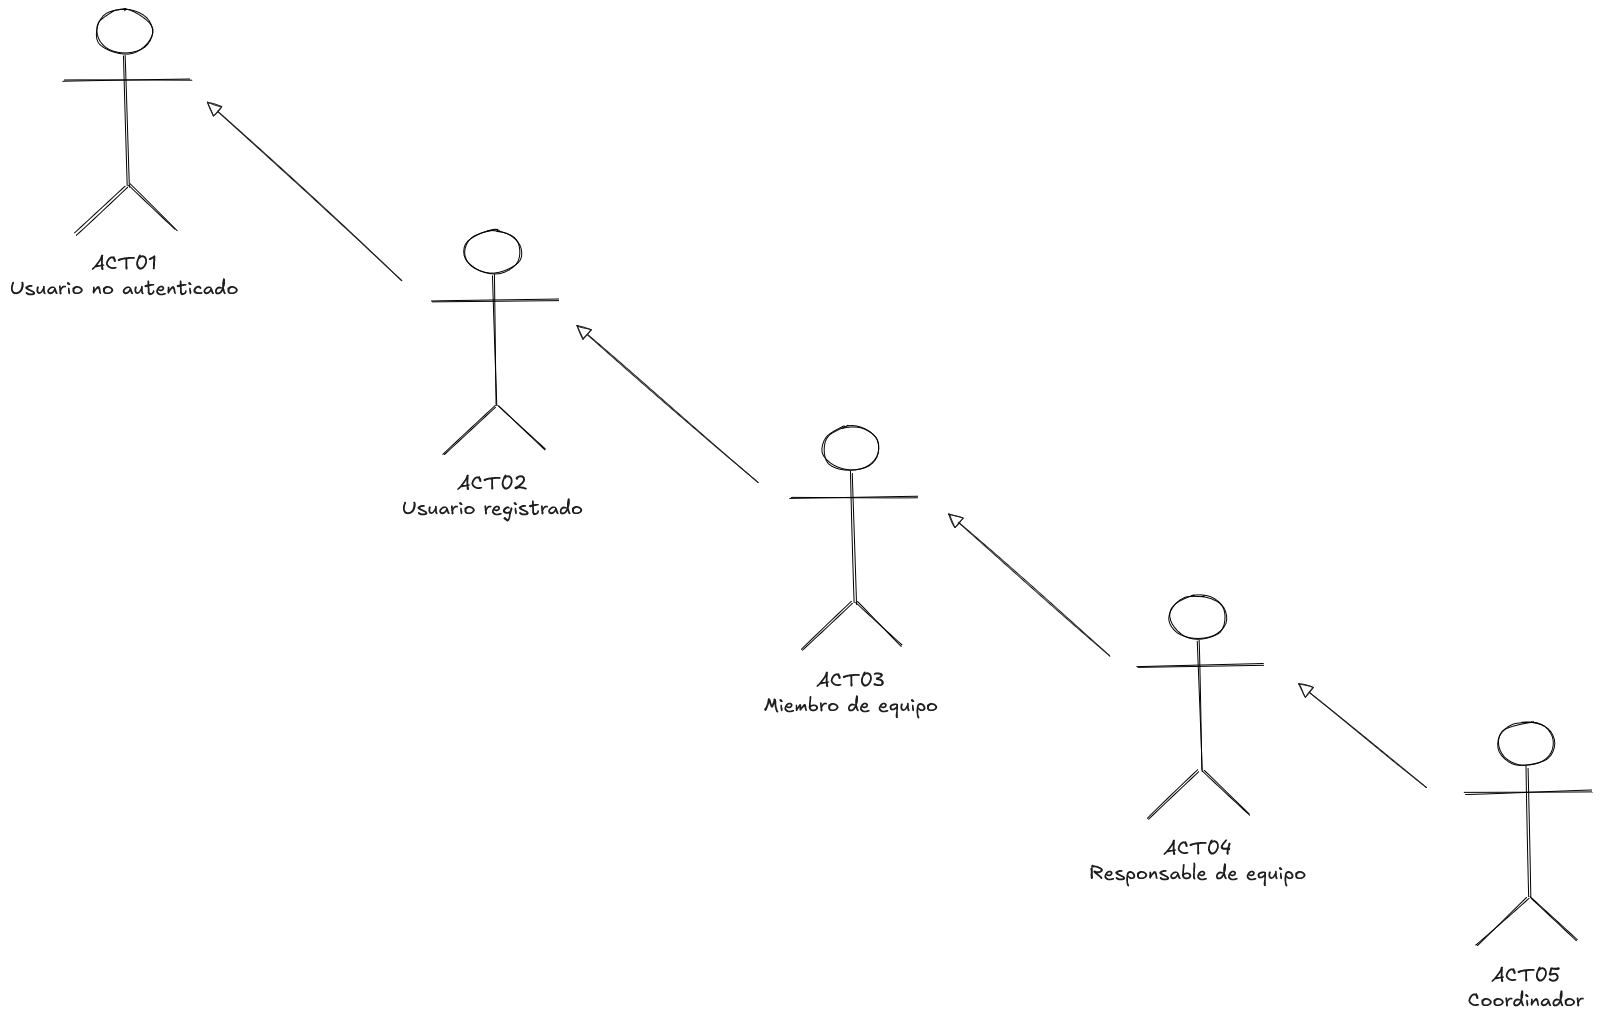
\includegraphics[width=1\textwidth]{imaxes/diagrama-actores.png}
  \caption{Diagrama de la jerarquía de actores del sistema}
  \label{fig:actores-sistema}
\end{figure}

Además, los permisos siguen una jerarquía acumulativa, como se muestra en la figura \ref{fig:actores-sistema}. Esto significa que cada actor superior hereda las capacidades del nivel anterior y añade nuevas funcionalidades. De este modo, el usuario no autenticado posee las capacidades más limitadas, entre ellas se encuentra la visualización del mapa de emergencias y la creación de avisos, mientras que el coordinador, a mayores de las funcionalidades de los roles anteriores cuenta con la capacidad de gestionar usuarios, organizaciones, emergencias y asignaciones, así como de configurar las reglas de recomendación para la asignación automática de recursos. Esta estructura jerárquica facilita la gestión de permisos y asegura que cada usuario tenga acceso únicamente a las funciones necesarias para su rol específico dentro del sistema.

\section{Casos de uso}

{ \color{red} Aspectos a considerar
    \begin{itemize}
      \item Agrupar casos de uso (servirá de base para agruparlos en servicios posteriormente en la sección de diseño).
      \item Definición concreta /detallada de cada caso de uso (precondiciones ...)
    \end{itemize}
}

\section{Modelo de casos de uso}

{ \color{red} Aspectos a considerar
    \begin{itemize}
      \item Diagrama de casos de uso incluyendo actores y relaciones entre casos
    \end{itemize}
}

\section{Prototipado de interfaz}

{ \color{red} Es interesante hacer el esfuerzo en este momento de prototipar las principales pantallas de la interfaz (y añadirlas en la memoria), como parte del análisis de requisitos, así como de aspectos de usabilidad de las mismas. }
